\section{Comparison of performances}
\subsection{Types of input}
When testing a topological input, we followed the Network Attribute Vector (NAV) approach of \cite{rosen2016topological,naaman2019edge}. In short, this approach presumes that the graph topological features (e.g. degree, clustering coefficient, centrality...) are correlated with the class of the node. As such these features can be used to predict the class of the node. We here deviate from this approach, by using the features as the input to a GCN, and letting the GCN combine these features with the adjacency matrix itself. For the NAV, we used the following topological features of each node: Attractor basin hierarchy \cite{muchnik2007self}, Flow measure \cite{rosen2014directionality} Average neighbor degree, Betweenness centrality, The first two moments of the distance distribution of each node to all other nodes, Closeness centrality, Eccentricity , Fiedler vector, K Core, Load centrality, Page Rank, and the frequency of small scale motifs surrounding each node, as proposed by Itzchack et al \cite{itzhack2007optimal}.
\\An alternative input is just using the trainning set node classification as an inputs. Formally, we count for each node the number of neighbors and second neighbors in the training set belonging to a class, leasding to a vector with twice the number of classes elements. We then tested each one of these inputs with or without the node information as inputs for different traning set fractions. We have thus tested the following 4 possible inputs:
\begin{enumerate}[A)]
\item   Topological features with inner content
\item   Topological features without inner content
\item   Neighbors data with inner content
\item   Neighbors data without inner content
\end{enumerate}
All the models outperform the results of JingFang et al (Figure \ref{fig:auc_inp_type}). The reuslts vary over the years, but the best results are for the combination of topology with external information, followed by the neighbors with internal information, followed by only the neighbor data, with a limited difference between the models, suggesting that the neighbor and topological infromation contain almost as much data as the detailed information in the balance sheets of the companies.

\begin{figure}[h!]
    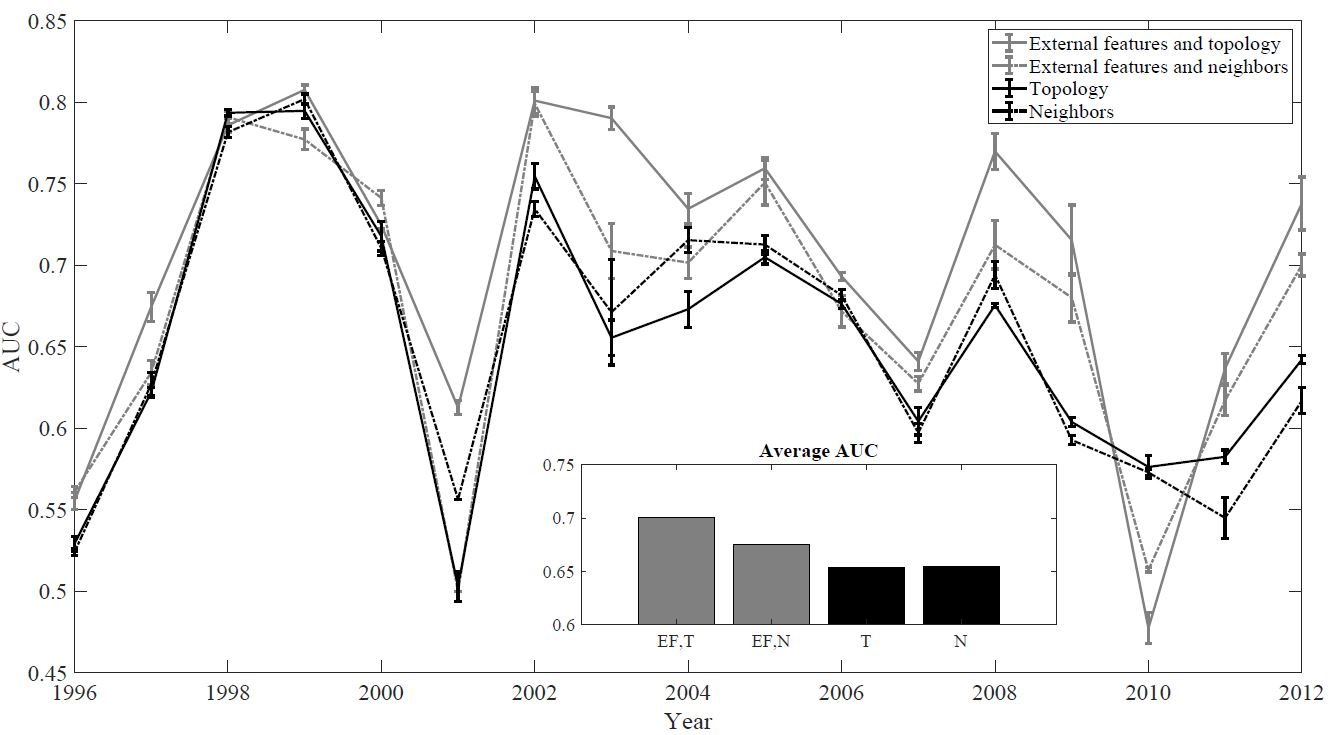
\includegraphics[width=\textwidth]{auc_inp_type}
    \centering
    \caption{\textit{Test AUC of the 4 types of input over the years and average (inset) for the first model. The gray lines use a combination of internal and topological information. The black lines use only topology. All models have a good accuracy in regular year (taking into account the complexity of predicting bankruptcy), but fail following crises (2000 and 2008). One can further notice that the models using the network topology and external information as input outperforms the others.}}
    \label{fig:auc_inp_type}
\end{figure}

\subsection{GCN-LSTM configration}
To test the effect of combining the GCN and LSTM we compared the different models above (Figure \ref{fig:auc_models_a}\ref{fig:auc_models_b}). The different models were trained either with or without internal information. Three interesting results emerge from the comparison. First, the precision varied significantly over the different years, and it drops following large scale crises to a random level (e.g. following the 2000 and 2008 crises). This may be the result of the large number of collapses that are not directly related to the regular market dynamics or the product portfolio. The second interesting result is that the combination with the RNN improves the performance, but the combined training of the GCN and the LSTM has a limited (yet significant) contribution to the accuracy. Moreover, the combined model is very sensitive to the initial conditions and often the loss does not converge to a low enough value. To resolve that, in the GCN-LSTM combined model, we performed multiple random initiations of the weights for a given training/test division. We then choose their realization with the best loss on the train. Finally, one can clearly see the effect of the LSTM in the crisis years, where the experience from a single year before is not enough to predict the collapse of companies, but the dynamic model manages to produce a better prediction. We have tested the same model for different types of input (as in the previous section) and different classifications with a similar ordering of the models (yet lower accuracies).
\\To further test the performance of the combined LSTM-GCN, we studied another network., where no external information was available. We again tested the 4 models using the topology as an input, and again the order of model performance is similar, with the GCN-LSTM drastically outperforming the GCN (Figure \ref{fig:auc_models_a}\ref{fig:auc_models_b}).
% \subsection{Combined model}
% HERE PLEASE CHECK A MODEL WHERE YOU DECIDE BASED ON THE TRAIN AUC WHETHER TO USE THE FULL MODEL OR WHETHER TO USE A SINGLE YEAR MODEL

\iffalse
\subsection{Types of input}
When testing a topological input, we followed the Network Attribute Vector (NAV) approach of
[24, 25]. In short, this approach presumes that the graph topological features (e.g. degree, clustering
coefficient, centrality...) are correlated with the class of the node. As such these features can be
used to predict the class of the node. We here deviate from this approach, by using the features as
the input to a GCN, and letting the GCN combine these features with the adjacency matrix itself.
For the NAV, we used the following topological features of each node: Attractor basin hierarchy
[26], Flow measure [27] Average neighbor degree, Betweenness centrality, The first two moments of
the distance distribution of each node to all other nodes, Closeness centrality, Eccentricity , Fiedler
vector, K Core, Load centrality, Page Rank, and the frequency of small scale motifs surrounding each
node, as proposed by Itzchack et al [28].
An alternative input is just using the training set node classification as an inputs. Formally, we count
for each node the number of neighbors and second neighbors in the training set belonging to a class,
leasding to a vector with twice the number of classes elements. We then tested each one of these
inputs with or without the node information as inputs for different training set fractions. We have thus
tested the following 4 possible inputs: A) Topological features with inner content, B) Topological
features without inner content, C) Neighbors data with inner content, and D) Neighbors data without
inner content. All the models outperform the results of JingFang et al (Figure 2). The reuslts vary
over the years, but the best results are for the combination of topology with external information,
followed by the neighbors with internal information, followed by only the neighbor data, with a
limited difference between the models, suggesting that the neighbor and topological infromation
contain almost as much data as the detailed information in the balance sheets of the companies.

When testing a topological input, we followed the Network Attribute Vector approach of (REF) and used the following topological features of each node: Attractor basin (REF),  Average neighbor degree, Betweenness centrality,  The first two moments of the distance distribution of each node to all other nodes,  Closeness centrality (REF), Eccentricity (REF), Fiedler vector (REF),  Flow measure (REF),  K Core (REF), Load centrality (REF), Page Rank (REF), and the frequency of small scale motifs surrounding each node (REF).
For stage 1 I ran 4 input scenarios:
•	Combined topological features with inner content
•	Combined topological features without inner content
•	Neighbors topological data with inner content
•	Neighbors topological data without inner content
As observed before, the best results came from the combination of topological features (all, including the neighbors, excluding motif4), with the inner data.
If we exclude the inner data, the neighbor's input achieved better than the combination of neighbors with topological features.
\fi
